\documentclass[10pt, oneside,spanish]{article}   	
\usepackage{geometry}
\usepackage{amsmath}
\geometry{a4paper}                   		
\usepackage[utf8]{inputenc}               	 \usepackage{listings}	


\usepackage{graphicx}												
\usepackage{amssymb}
\usepackage{authblk}




\linespread{1.45}

\title{MKTG 212 - Case 3: Conjoint Analysis} \lstset{language=R}

\author[]{Juan Manubens}

\affil[]{University of Pennsylvania}
\renewcommand\Authands{, }
\date{}							
\begin{document}
\maketitle







\section{Conjoint Study}

\textit{Gidi, the Marketing Research Man (GMRM), is considering a launch of a new type of raisin into the packaged raisin market.  Prior to launch, however, GMRM has decided that a conjoint study of potential consumers might be useful to help in his product design.  Even though Gidi knows marketing research, he wants a second opinion. Pretend that you are a marketing research company hired to provide GMRM help with the following issues.}

\begin{itemize}
\item \textbf{[1a] GMRM would like to make sure he has the right attributes and levels of those attributes to include in the conjoint study.  Please provide a step-by-step process (with at most five steps) that GMRM can employ to get the right conjoint attributes and their levels.  }
\end{itemize}

\begin{enumerate}
\item Analyze the market and competition - Understand the size of the market, target customers, and who the main competitors. Identify the attributes and their levels for the main competitors’ product. 
\item Pilot studies (open ended surveys, ratings, ranking) to determine attributes to include, make sure they are unambiguous, actionable and useful for determining choice or preference (on average 6 attributes)
\item Conduct qualitative research to decide on appropriate attribute levels. 
\item Set an empirical range in product category to determine range of attributes
\item Determine which format of conjoint analysis you want to use - ratings-based conjoint or choice-based conjoint
\end{enumerate}





\begin{itemize}
\item \textbf{[1b] How would you validate that the attributes and levels you obtained are an “appropriate” set?}
\end{itemize}
\begin{enumerate}

\item Confirm determined attributes with the results from pilot studies conducted before.

\item Ensure that the attributes selected are unambiguous, mutually exclusive, and actionable, and through surveys and market research make sure they are not "must-have" attributes.




\end{enumerate}

\textbf{After GMRM heard your answer to (1a), he went out and collected product ratings on a 1-10 Likert-scale from consumers utilizing the following attributes and corresponding levels,}

\begin{center}
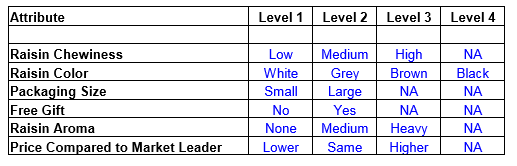
\includegraphics[width=8cm]{q1.PNG}
\end{center}

\textbf{where NA indicates not applicable (e.g. Chewiness has only three levels).  The data that GMRM collected is sitting in canvas (conjoint data).  Please base your answer to the following questions on this data.  Note that each attribute is coded numerically.  For instance, for Chewiness (Low =1, Medium =2, High =3) and similarly for the other attributes reading left to right in the table above. (Hint: GMRM remembers that one has to create dummy (0/1) variables to represent the different levels of attributes.)}

\textbf{For the following questions, assume a homogeneous market (ignore the segment variable for now). }


\begin{itemize}
\item \textbf{[1c] Determine the relative percentage importance of each attribute.}
\end{itemize}

We computed the relative importance of each attribute by summing the ranges of their respective coefficients (including, of course, the 0-coded coefficient too), and computing the fraction each of the attribute-ranges made up of this sum. The relative percentage importance is summarized below:

\begin{itemize}
\item Chewiness: 21.85\%
\item Color: 12.11\%
\item Size: 22.69\%
\item Free Gift: 2.31\%
\item Aroma: 24.51\%
\item Price: 16.52\%
\end{itemize}



\begin{itemize}
\item \textbf{[1d] What Likert  rating score would you predict for a raisin product that has Low Chewiness, Grey Raisins, Large Package Size, Free Gift, Medium Aroma, and the Same Price as the Market Leader?  You may round your answer to the nearest integer. }
\end{itemize}

\begin{center}
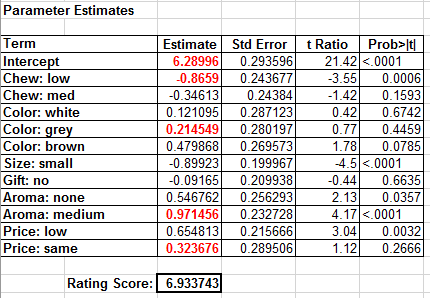
\includegraphics[width=8cm]{1d.PNG}
\end{center}

Multiplying the applicable dummy variables by 1 and adding them to the intercept, we arrive at the following predicted Likert score:

6.93  - rounded to 7

\begin{itemize}
\item \textbf{[1e] What product has the highest predicted rating score}
\end{itemize}

A raisin product with (a) High Chewiness, (b) Brown, (c) Free Gift-Yes, (d) Aroma-Medium, (e) Lower Price, (f) Large Package Size has a rating score of 8.40.


\begin{itemize}
\item \textbf{[1f] Would you necessarily introduce this product, the one from (1e) if you were GMRM?  Why or why not?}
\end{itemize}

Not necessarily. There are many possible reasons why it might not make sense to introduce the product. For example, the combination of the low price and the desirable product attributes (which are likely more costly), might seriously reduce the profit margin of the product. It could also be the case that certain of the attributes do not go well together, i.e. the attributes are individually desirable but not desirable as a bundle, or there is a negative interaction effect. 

\begin{itemize}
\item \textbf{[1g] Suppose that the market currently contains the following three products:}
\end{itemize}

\textbf{(A)	High Chewiness, Grey Raisins, Small Package Size, No Free Gift, Medium Aroma, and Same Price as Market Leader
(B)	Low Chewiness, Brown Raisins, Small Package Size, Free Gift, Medium Aroma, and Same Price as Market Leader
(C)	Medium Chewiness, Black Raisins, Large Package Size, No Free Gift, No Aroma, and Lower Price as Market Leader, and that the predicted market share of product j is proportional to Rj; that is market share = $Rj/j'Rj'$ where $Rj$ is the predicted Likert rating of product $j$.  What would the predicted market share be if the product described in (1d) were introduced into the market consisting of current products A,B,C?} 

\begin{itemize}
\item Product A has an estimated Likert score of 6.81
\item Product B has an estimated Likert score of 6.30
\item Product C has an estimated Likert score of 7.05
\item Product from 1D has an estimated Likert score 6.93
\end{itemize}

The sum of the estimated scores is 27.10. Accordingly, the predicted market shares are, $$M_A = 25.13\% (A) , M_B = 23.25\% , M_C = 26.03\% , \quad \textrm{and} \quad M_{1d} = 25.59\% $$


\begin{itemize}

\item \textbf{[1h]  Suppose that the market for raisin products, in total, is 60 Million Dollars and that if GMRM had not hired the market research firm he would have introduced the product in (1d) into the market with the three existing products. Assuming GMRM paid the market research firm \$1,500,000 for their services and that as a result of running the conjoint study, he would introduce the best product, i.e. the product that you found in question (1e) not the one in (1d), was the market research firm worth the money that was paid to them?  Justify your answer.   }
\end{itemize}

With the superior product in 1e and an estimated Likert score of 8.39, GMRM's raisin product would have a market share of 29.40\%.

As such, the net revenue of the two products would be:
\begin{itemize}
\item $Product_{1d}: $ \$60MM * 25.59\% = \$15.354MM
\item $Product_{1e}: $ \$60MM * 29.40\% - \$1.5MM = \$16.140MM

\end{itemize}

	
    
    
Thus, the product of question 1e is more attractive by a net difference of \$786,144. In other words, the marketing research paid off.


\begin{itemize}
\item \textbf{[1i] Do the product attributes (as a whole) provide significant predictive power for the rating scores?  Justify your answer.    }
\end{itemize}


The Omnibus $F$-statistic for significance is less than .0001 (see Appendix 3.1) at a $\alpha = 0.05$ significance level ($F$-ratio $ = 5.9763 $) . Therefore, this mix of product attributes as a whole does provide significant predictive power for the rating scores. 

\begin{itemize}
\item \textbf{[1j]   Which, product attributes, if any, have no statistically significant explanatory power for rating scores?  State clearly how you arrived at your answer.  }
\end{itemize}



Our results show that the color attribute is not significant at any level, and the free gift variable isn't either (see Appendix 3.1). This can be inferred from the $p$-values which are statistically significant if below 0.05 (and highlighted in orange/red, accordingly). 

The chewiness attribute is only significant on its difference between low chewiness and high chewiness, but it is not significant on its difference between medium chewiness and high chewiness.  Similarly, price is not significant on same as market as compared to higher than market price; it is only statistically significant in the difference between lower and higher than market. 

The product attributes that have statistically significant explanatory power for all levels are the package size and aroma.



\begin{itemize}
\item \textbf{[1k] For each segment, determine the percentage importance for each attribute.  How do the segments differ? Please be specific.     }
\end{itemize}

(See Appendix 3.2 for calculations)


\textbf{Segment 1:}
\begin{itemize}
\item Chewiness: 22.29\%
\item Color: 7.97\%
\item Size: 18.52\%
\item Free Gift: 3.74\%
\item Aroma: 30.86\%
\item Price: 16.63\%
\end{itemize}

\pagebreak

\textbf{Segment 2:}
\begin{itemize}
\item Chewiness: 18.47\%
\item Color: 15.90\%
\item Size: 30.75\%
\item Free Gift: 5.91\%
\item Aroma: 17.33\%
\item Price: 11.65\%
\end{itemize}

The segments differ in that Segment 2 deems size by far the most important attribute at 30.75 percent, whereas Segment 1 has size as the third most important attribute, at a mere 18.52 percent.  For its part, Segment 1 considers aroma to be the most important attribute, at 30.86 percent, while Segment 2 has aroma as the third most important, at 17.33 percent.  Other differences are that Segment 1 considers chewiness to be a somewhat more important (22.29 percent vs. 18.47 percent), color to be considerably less imporant (7.97 percent vs. 15.90 percent), the presence of a free gift to be about the same in importance (3.74 percent vs. 5.91 percent), and price to be a bit more important (16.63 percent vs. 11.65 percent) than Segment 2 does.   

\begin{itemize}
\item \textbf{[1l]   For each segment, what Likert  rating score would you predict for a raisin product that has Low Chewiness, Grey Raisins, Large Package Size, Free Gift, Medium Aroma, and the Same Price as the Market Leader?    }
\end{itemize}

For segment 1, this product would have an expected Likert score of 7.094

For segment 2, this product would have an expected Likert score of 6.702

\begin{itemize}
\item \textbf{[1m]   For each segment, which product has the highest predicted rating score?    }
\end{itemize}

For segment 1, the combination which yields the highest predicted rating score is: (a) high chewiness, (b) brown color, (c) large package size, (d) no free gift, (e) medium aroma, and (f) lower price.

For segment 2, the combination which yields the highest predicted rating score is: (a) high chewiness, (b) brown color, (c) large package size, (d) free gift, (e) medium aroma, and (f) lower price.

In other words, regardless of the differences of importance as described in question 1L, only one variable changes in terms of yielding the highest predicted Likert score between the two segments: whether or not a free gift is included.
\pagebreak


\section{Survey Analysis}

\textit{In addition to the conjoint study that was done, GMRM also decided that it would be useful to survey a sample of supermarket owners for their opinions on the raisin industry.  To conduct this survey, GMRM constructed a list of names containing the largest 200 supermarket owners who had email accounts.  He then conducted an email study in which these supermarket owners were sent a questionnaire with 10 items on it regarding the raisin category in their supermarket.  Out of the 200 supermarket owners emailed, 120 responded, for a response rate of 60\%.  The 10 questions asked of the supermarket owners are located at the website above and are labeled “supermarket owner questionnaire”, and their responses are labeled “survey data with item non-response.txt”.  Note that some of the questions were not answered by some of the supermarket owners; hence the item non-response (labeled as ‘.’).  Based on this information, please answer the following questions.}

\begin{itemize}
\item \textbf{[2a]  List three potential biases in the way that this study was conducted.   }
\end{itemize}

\textbf{Possible biases:}

\begin{enumerate}
\item Selection Bias - The sample of the 200 supermarket owners emailed does not reflect the population of supermarket owners.  Because only the largest supermarket owners who had email accounts were surveyed, this leaves out small businesses or supermarket owners that don't use email.  The circumstances and observations of small and large businesses are often different, which renders this survey skewed toward larger and more technological advanced supermarkets. 

\item Response Bias - Perhaps the observations of the 120 respondants do not reflect the observations of the 200 supermarket owners emailed.  The circumstances and observations of the businesses that respond are often very different from those that don't. (For example, if the reason that some owners didn't respond to the survey is that their business is too busy, their answers had they responded would probably have significantly differed than the recorded responses.)  Indeed, not all the questions were answered by all the survey participants, so some questions' responses only represent a certain group of owners. 

\item Anchoring effect from Order and Leading Question bias: The subjects' response may depend in the order in which they are asked the questions in the survey. Similarly, through statements like  'Raisin sales are highly linked to the sales of other fruits.' included in the questionnaire, some respondents may be encouraged to say they agree more than they would if the statement didn't contain words like "highly." For instance, another way to phrase the question could be "On a scale from 1 to 10, how linked are raisin sales to the sales of other fruits?" 
\end{enumerate}

\begin{itemize}
\item \textbf{[2b]   GMRM decided to delete all observations with any missing data. Based on the data set with all such observations deleted, which variables (out of Q1-Q9) are significant predictors, at the 10\% significance level, of Q10, the overall profitability in the raisin category?  Justify your answer.  }
\end{itemize}

We cleaned the data using R (code and results in Appendix 3.4 and 3.5 respectiveley), and ran a Multi-variable OLS regression on the clean data set, using $X: Q_1, ... , Q_9$ and $Y: Q_{10}$. As we can see, at $\alpha = 0.1 $, $X^{*}: Q_1,Q_3, Q_4, Q_7,Q_8 \quad \textrm{and} \quad Q_9 $ are significant predictors for $Y: Q_{10}$ 

\begin{itemize}
\item \textbf{[2c]   Suppose that GMRM decides to use a sophisticated method to fill in the missing values.  The data set, filled in by stochastic imputation is located on Canvas (“Sophisticated imputation survey data.txt”).   Re-run your model with this data set and compare and contrast your answers to that from questions (2b).  What are the main findings? Any differences inform us about how deleting missing data can have an impact on the main findings.  }
\end{itemize}

The main findings are that running a least squares regression, all variables except Q5 and Q6 are significant at the 10 percent level. Before, Q2 wasn't a significant variable, and Q1 and Q4 had larger p-values (were less significant).  When missing data is deleted, less information is available in the model (because there are fewer observations compared to when all data is present), which means the variables are less predictive.
   

\begin{center}
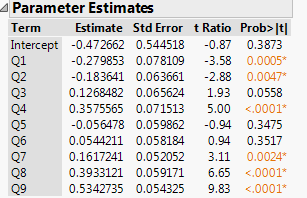
\includegraphics[width=8cm]{2c.PNG}
\end{center}

\pagebreak

\begin{itemize}
\item \textbf{[2d]  Imagine that for each of the 120 supermarket owners, you also had information from the three questions listed at the end of the questionnaire.  List three ways in which that information could be used for target marketing and/or inferential purposes.   }
\end{itemize}

(See Appendix 3.3 for the Questionnaire)

Answers to the question "How many different SKUs of raisins does your store carry?" could be the first question to ask when trying to find out whether stores would carry different types of raisins we could launch or would rather keep things simple and only carry the basics.  This could be used to figure out which stores to target for distribution becuase it would tell you which stores are focused on selling raisins and which aren't.  It could also be viewed alongside the attribute importances of the consumers that shop in these stores in order to determine if the store is carrying the type of raisins its customer desires or falling short and would benefit from selling more types of our raisins.  

Answers to the question "What is the monthly dollar volume of your store?" could be used to figure out if there's a relationship between store size and customer preferences.  For example, perhaps customers that shop in smaller stores go there for varieties of raisins not carried in larger chains.  The question could also indicate where would be the best exposure if we wanted to test launch a new type of raisin, because it shows where the most people will see it.

Finally, answers to "How much marketing expenditure, per month, do you spend on the raisin category?" can be used to determine the importance stores place on marketing their raisins and whether this affects customer preferences.  If, for example, one store spent a lot on raisin marketing, perhaps their customers' preferences would align with the raisin characteristics advertised by the store.  In addition, if a store spends a lot of money on raisin marketing, it will likely benefit us to place our products there because they're more likely to be purchased by the consumers who see the advertisements.

\pagebreak

\section{Appendix}

\subsection{JMP Outputs for Q1(i,j)}

\begin{center}
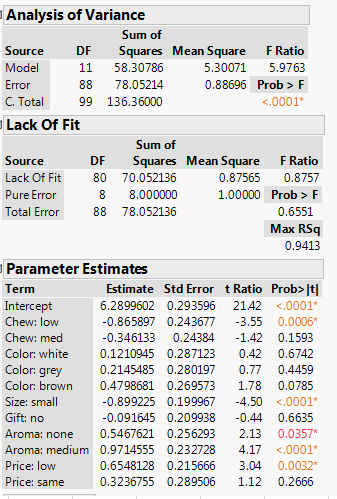
\includegraphics[width=8cm]{1j.PNG}
\end{center}


\subsection{Calculations for Q1(k)}

\begin{center}
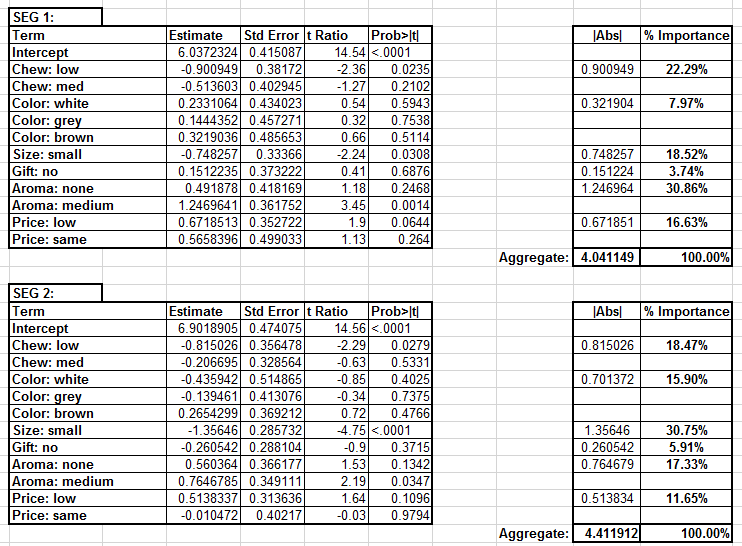
\includegraphics[width=14cm]{1k.PNG}
\end{center}

\pagebreak

\subsection{Supermarket Owner Questionnaire}


Please answer each of the following questions on a 1-10 scale where 1 indicates that you disagree completely with the given statement and 10 indicates perfect agreement.
\begin{enumerate}


\item Raisin color is a key determinant of raisin category sales.
\item Raisin aroma is a key determinant of raisin category sales.
\item Raisin consumers have differing preferences for varying raisin package sizes.
\item Giving away in-package free gifts is a strong driver of brand sales.
\item Raisin consumers are price sensitive.
\item Raisin chewiness is an important determinant of raisin preference.
\item Raisin sales are highly linked to the sales of other fruits.
\item Marketing for the raisin category can significantly affect people’s purchasing habits.
\item I enjoy raisins as part of my daily diet.
\item The raisin category is extremely profitable in my store.

\end{enumerate}

Additional Questions: 

What is the monthly dollar volume of your store?
How much marketing expenditure, per month, do you spend on the raisin category?
How many different SKUs of raisins does your store carry?

\pagebreak

\subsection{Q2(b,c) R Code for Data-cleaning }



\begin{center}
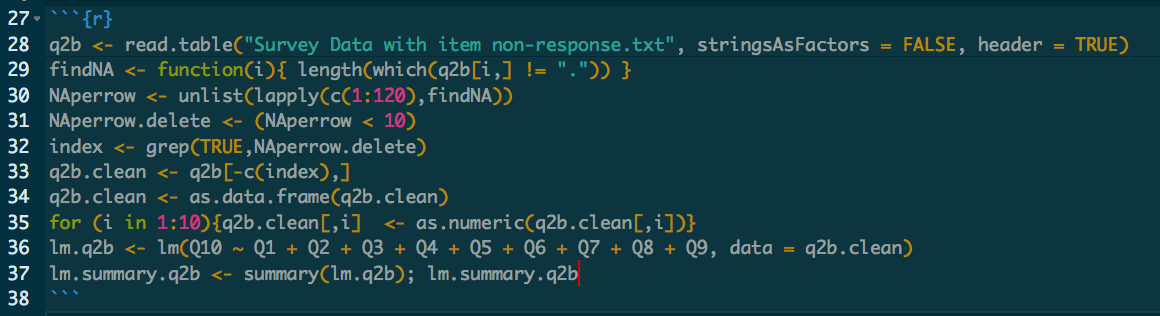
\includegraphics[width=16cm]{q2bcode.png}
\end{center}



\subsection{Q2(b) R Output }
\begin{center}
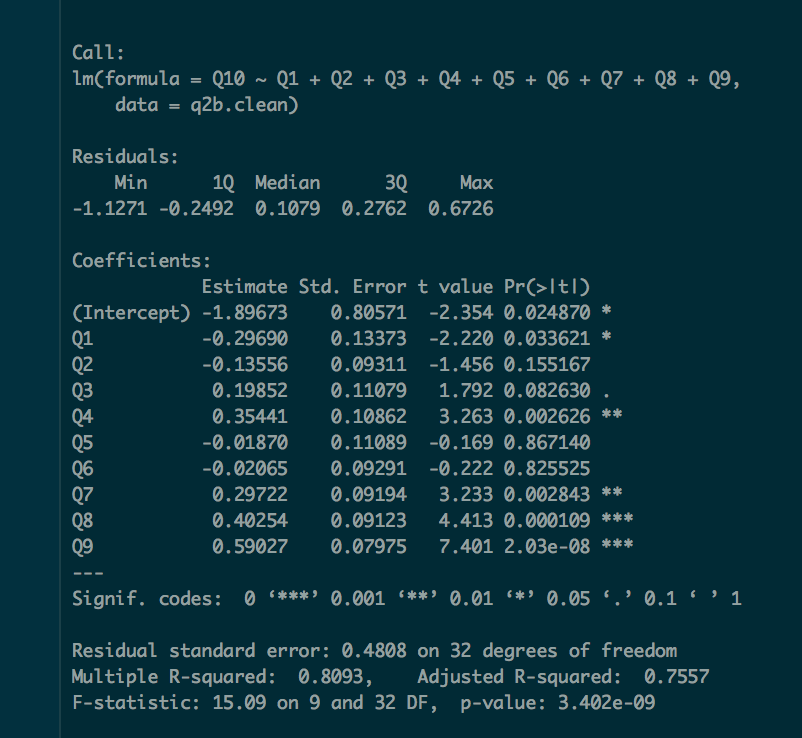
\includegraphics[width=14cm]{q2b.png}
\end{center}


\end{document}   
